\documentclass{article}
\usepackage{graphicx}
\usepackage{caption}
\usepackage{subcaption}
\usepackage{hyperref}
\graphicspath{{./figs/}}{}
\usepackage{listings}
\title{
HLS-Assignment 9 PART-1
}
\begin{document}
\maketitle
\hfill \textbf{Sampath Govardhan} \\
\null \hfill \textbf{FWC22071}\\
\maketitle
\hfill \textbf{VITIS-HLS}
\section{Problem Statement}
\href{run:./problem_statement.pdf} {Problem Statemt}
\vspace{1cm}
\section{Header File}
\begin{lstlisting}
//header.h
#ifndef _HEADER_H_
#define _HEADER_H_

#include <hls_stream.h>
#include "ap_int.h"
using namespace std;

#define N 8      //length of input message
#define y 25     //length of divisor(parity)
#define x N+y-1  //length of crc (len of input+divisor-1)

typedef ap_uint<N> data;


void crc24a(hls::stream<data>& input, hls::stream<data>& output, ap_uint<1> last);

#endif



\end{lstlisting}

\vspace{15cm}
\section{CRC bits Generator Code}
\begin{lstlisting}
//crc.cpp
#include "header.h"

void crc24a(hls::stream<data>& input, hls::stream<data>& output, ap_uint<1> last) {

#pragma HLS INTERFACE mode=axis register_mode=both port=input register
#pragma HLS INTERFACE mode=axis register_mode=both port=output register
#pragma HLS INTERFACE mode=ap_none port=last

	ap_uint<1> crc[x];
    ap_uint<1> divisor[y] = {1, 1, 0, 0, 0, 0, 1, 1, 0, 0, 1, 0, 0, 1, 1, 0, 0, 1,
    1, 1, 1, 1, 0, 1, 1};


// Read input stream a
    data d =input.read();
        for (int j = 0; j < N; j++) {
#pragma HLS PIPELINE II=1
            crc[j]=d[j];
        }
// Add padding zeros to message
    for (int i = 8; i < x; i++) {
#pragma HLS PIPELINE II=1
        crc[i] = 0;
    }


// Division is performed only when last is high
    for (int i = 0; i <= x - y; i++) {
#pragma HLS PIPELINE II=1
        if (crc[i] == 1  && last==1) {
            for (int j = 0; j < y; j++) {
#pragma HLS UNROLL
                crc[i + j] = crc[i+j] ^ divisor[j];
            }
        }
    }

// Find start index of nonzero bits in crc
    int startIdx = 0;
    while (startIdx < x && crc[startIdx] == 0) {
        startIdx++;
    }

// Store nonzero values into another array and minimum length will be length of divisor-1
	ap_uint<1> temp[y-1];

    for (int i = 0; i < y-1; i++) {
#pragma HLS PIPELINE II=1
    	temp[i] = (startIdx == x) ? crc[i] : crc[startIdx + i];
    }

// Write the result to output stream c
   data o1,o2,o3,o4;

   for (int i = 0; i < y-1; i++) {
#pragma HLS PIPELINE II=1
          if (i < N) {
              o1(i, i) = d(i, i);
              o2(i, i) = temp[i];
          } else if (i < N*2) {
              o3(i%N, i%N) = temp[i];
          } else {
              o4(i%N, i%N) = temp[i];
          }
      }

    output.write(o1);
    output.write(o2);
    output.write(o3);
    output.write(o4);

}

\end{lstlisting}
\vspace{13cm}

\section{Test Bench Code}
\begin{lstlisting}
//crc_tb.cpp
#include "header.h"

int main() {
    hls::stream<data> a,b;
    data w, z;
    ap_uint<1> last;

      w=0b00010110;                                               //msbtolsb

          /* ap_uint<1> dividend[8] = {0, 1, 1, 0, 1, 0, 0, 0};   //lsbtomsb
   	       for (int i = 0; i < 8; i++) {

   	              w(i,i) = dividend[i];

   	              }
   	      */

   	       a.write(w);
   	       last=1;



// Perform binary divison
    crc24a(a, b, last);

// Read the result from the output stream out1
    cout << "CRC generator output : ";
    ap_uint<1> p[32];


    for (int i = 0; i < 4; i++) {
        z = b.read();
        for (int j = 0; j < 8; j++) {
            p[i * 8 + j] = z(j, j);
        }
    }

    for (int i = 0; i < 32; i++) {
        cout << p[i];
    }

    cout<<endl;

// Checking if output is valid or not
    ap_uint<1> comp[32]; bool flag=0;
    ap_uint<1> divisor[y] = {1, 1, 0, 0, 0, 0, 1, 1, 0, 0, 1, 0, 0, 1, 1, 0, 0, 1,
    1, 1, 1, 1, 0, 1, 1};


//Output is valid only when remainder divison of output with divisor is 0
    for (int i = 0; i <= x - y; i++) {
        if (p[i] == 1) {
            for (int j = 0; j < y; j++) {
                p[i + j] = p[i+j] ^ divisor[j];
            }
        }
    }
    cout<<"CRC detector output :  ";
    for (int i = 0; i < 32; i++) {
    	cout<<p[i];
        if (p[i]==1){
        	flag=1;
        }
    }
     cout<<endl;
    if ( flag==0) {
               cout << "!PASS!CRC Check at detector is Success" << std::endl;
           }
    else {
               cout << "!ERROR!CRC Check at detector has Failed" << std::endl;
           }
    return 0;
}
\end{lstlisting}
\vspace{13cm}


\section{C simulation Output}
\begin{lstlisting}
INFO: [SIM 2] *************** CSIM start ***************
INFO: [SIM 4] CSIM will launch GCC as the compiler.
   Compiling ../../../../codes/crc_tb.cpp in debug mode
   Compiling ../../../../codes/crc.cpp in debug mode
   Generating csim.exe
CRC generator output : 01101000101101001111001100000010
CRC detector output :  00000000000000000000000000000000
!PASS!CRC Check at detector is Success
INFO [HLS SIM]: The maximum depth reached by any hls::stream() instance in the design is 4
INFO: [SIM 1] CSim done with 0 errors.
INFO: [SIM 3] *************** CSIM finish ***************



\end{lstlisting}
\vspace{15cm}

\section{HLS Resource Consumption Report}
\vspace{1cm}
\begin{figure}[h]
\centering
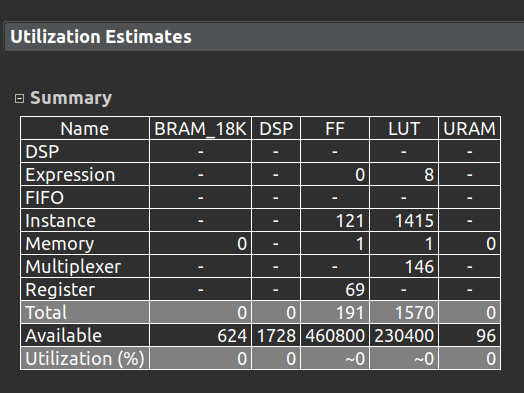
\includegraphics[width=\textwidth]{figs/p11.png}
    \caption{Resource Consumption}
    \label{fig:my_label}
\end{figure}

\vspace{13cm}


\section{HLS Timing and Fmax Report}
\vspace{1cm}
\begin{figure}[h]
    \centering
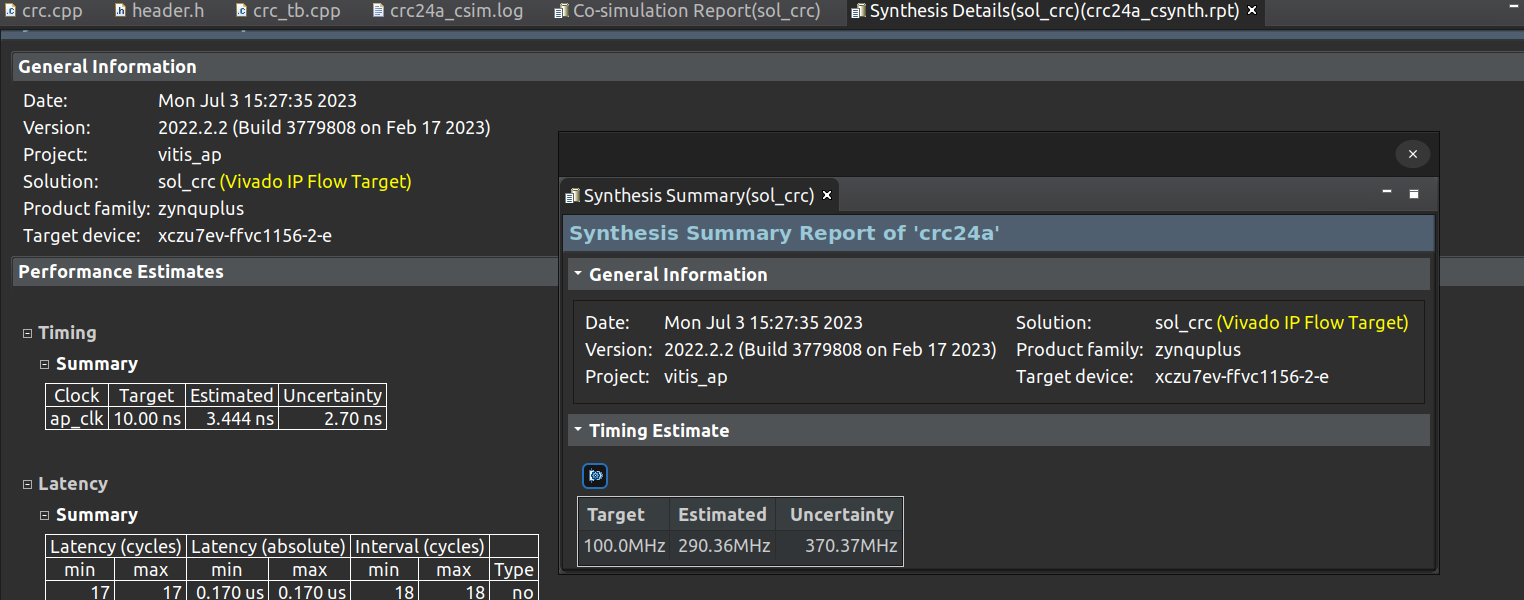
\includegraphics[width=\textwidth]{figs/p12.png}
    \caption{Timing and Fmax}
    \label{fig:my_label}
\end{figure}

\vspace{15cm}


\section{CoSimulation Report}
\vspace{1cm}
\begin{figure}[h]
    \centering
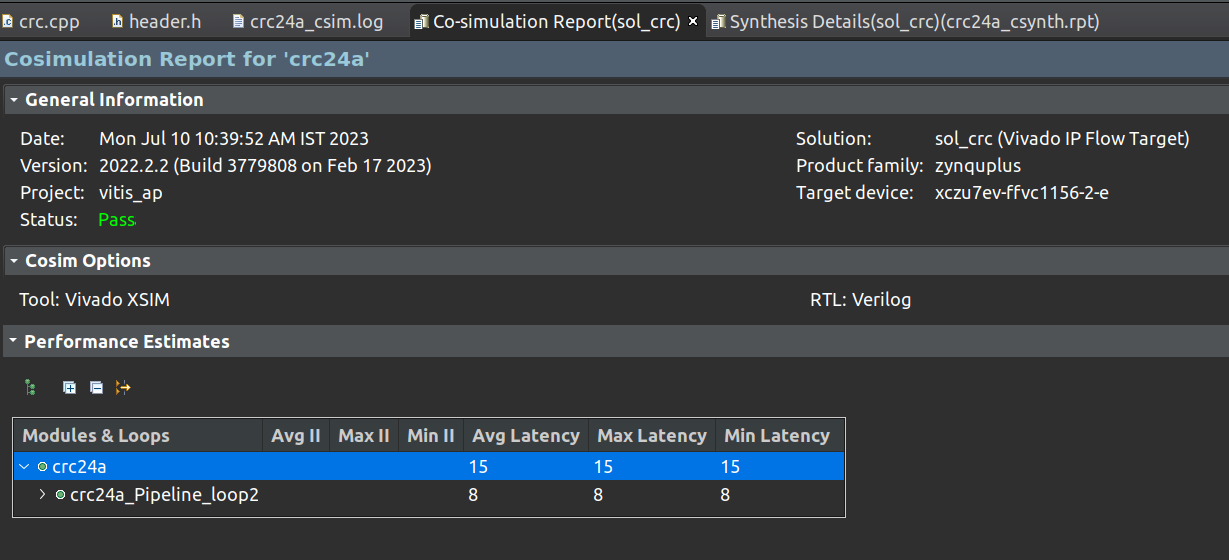
\includegraphics[width=\textwidth]{figs/p13.png}
    \caption{Cosimulation}
    \label{fig:my_label}
\end{figure}

\vspace{15cm}


\maketitle
\hfill \textbf{VIVADO}
\section{Block Design}
\vspace{1cm}
\begin{figure}[h]
    \centering
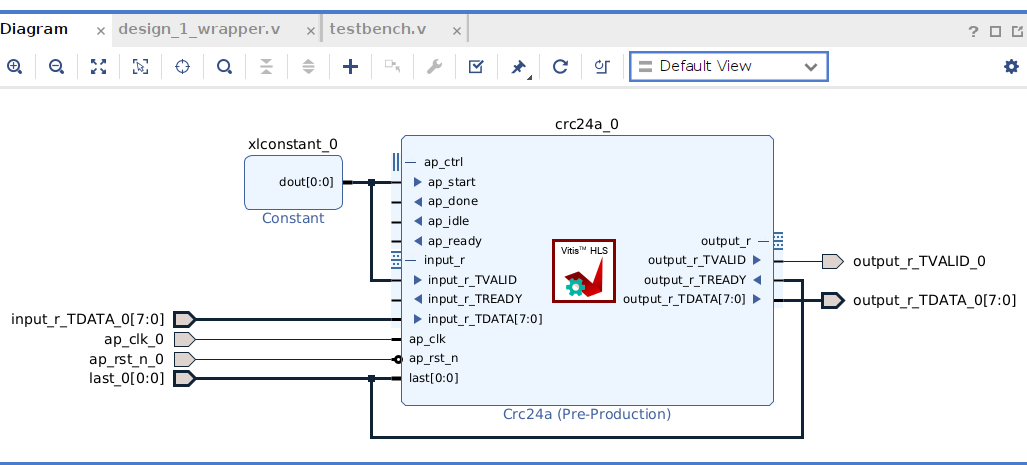
\includegraphics[width=\columnwidth]{figs/p1bd.png}
    \caption{Block Diagram}
    \label{fig:my_label}
\end{figure}
\vspace{3cm}
\section{Verilog Testbench}
\begin{lstlisting}
//testbench.v
`timescale 1ns / 1ps
//////////////////////////////////////////////////////////////////////////////////
// Company: 
// Engineer: 
// 
// Create Date: 06/26/2023 11:35:30 AM
// Design Name: 
// Module Name: testbench
// Project Name: 
// Target Devices: 
// Tool Versions: 
// Description: 
// 
// Dependencies: 
// 
// Revision:
// Revision 0.01 - File Created
// Additional Comments:
// 
//////////////////////////////////////////////////////////////////////////////////


module testbench();
        reg ap_clk_0;
        reg ap_rst_n_0;
        always #5 ap_clk_0=~ap_clk_0;
        
        reg [7:0] ip;
        reg last_0;
        wire [7:0] op;
        wire output_r_TVALID_0;
       
        initial begin
        ap_clk_0=0;ap_rst_n_0=0;
        #10
        ap_rst_n_0=1;
        #10
        ip=16'b00010110;//ascii "h"

        #1  last_0=1;
        #2000
        $finish;
        end
     
     design_1_wrapper
     uut(.ap_clk_0(ap_clk_0), .ap_rst_n_0(ap_rst_n_0),.input_r_TDATA_0(ip),
     .last_0(last_0),.output_r_TDATA_0(op),.output_r_TVALID_0(output_r_TVALID_0));
    
    
endmodule

\end{lstlisting}

\vspace{3cm}


\section{Output Waveform}
\vspace{1cm}
\begin{figure}[h]
\centering
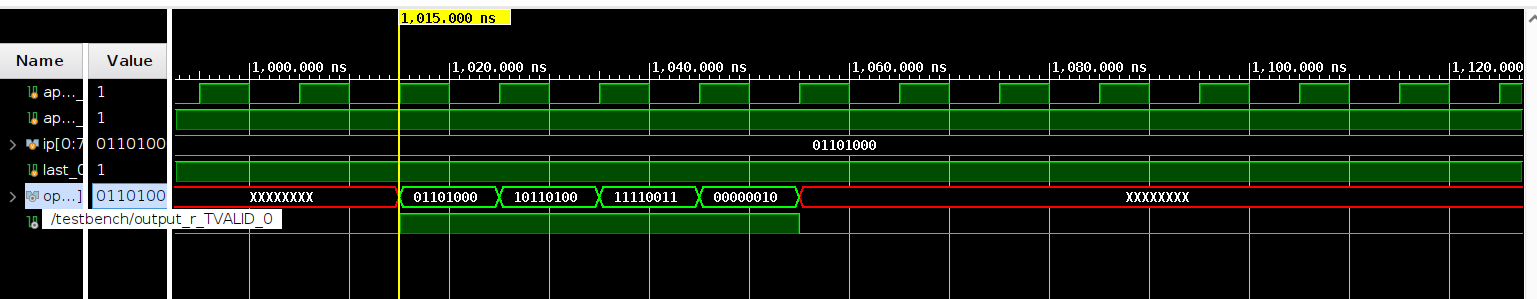
\includegraphics[width=\columnwidth]{figs/p1wav.png}
    \caption{Output Waveform}
    \label{fig:my_label}
\end{figure}
\vspace{15cm}

\maketitle
\hfill \textbf{MATLAB}
\section{Matlab Reference}
\begin{figure}[h]
\centering
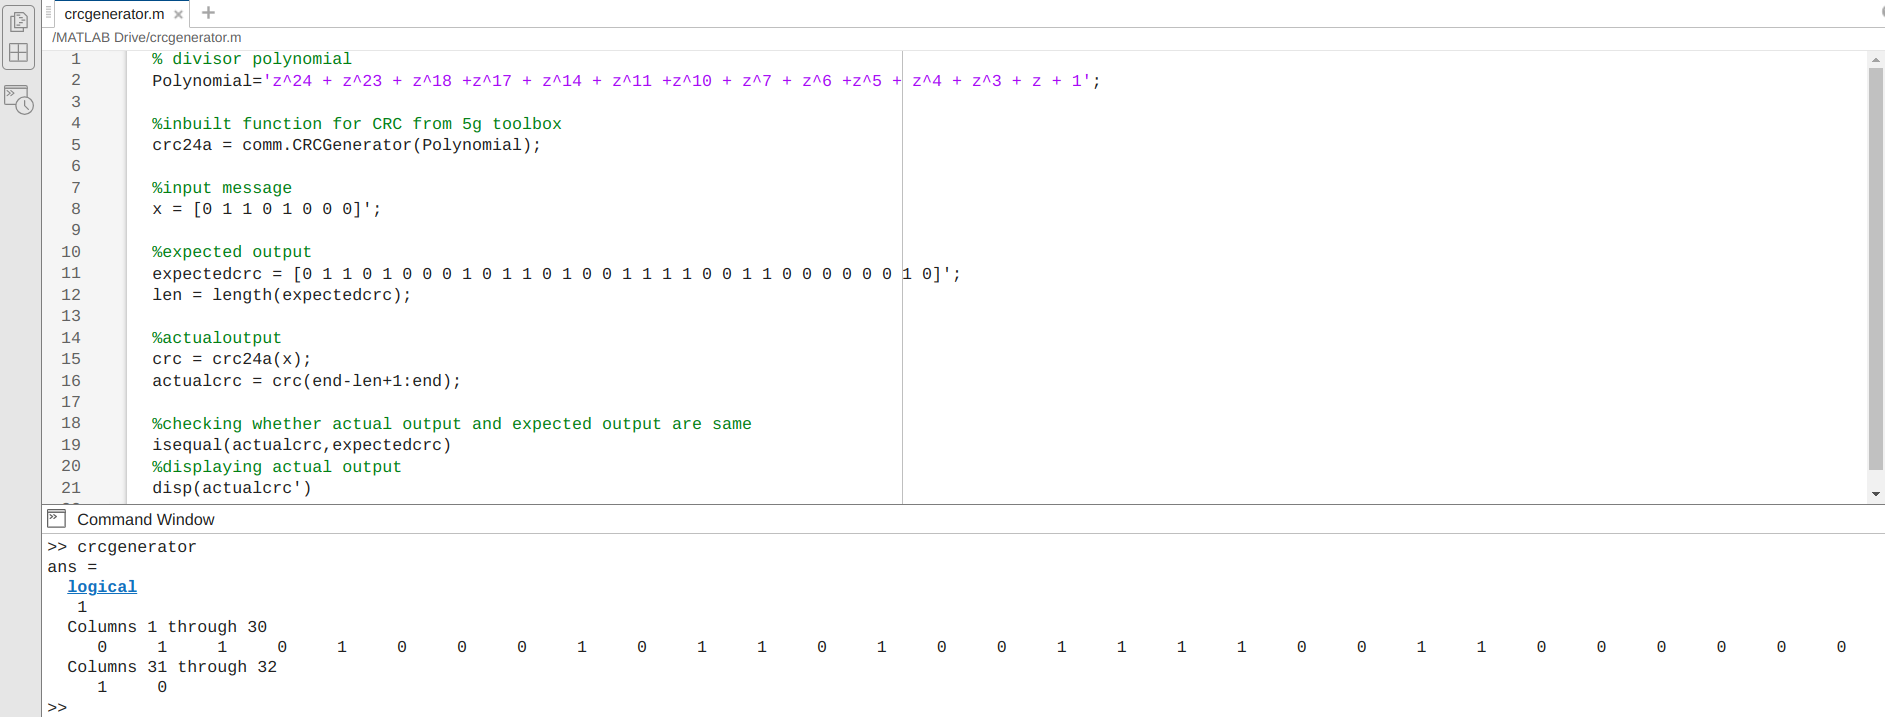
\includegraphics[width=\columnwidth]{figs/actual_matlab.png}
    \caption{Matlab Reference}
    \label{fig:my_label}
\end{figure}
\vspace{3cm}
\section{Conclusion}
\begin{lstlisting}
The Output of FFTIP is matching with Output of reference Matlab code and also
using this floating Point Converter Online :

\end{lstlisting}
\url{https://www.h-schmidt.net/FloatConverter/IEEE754.html}
\vspace{4cm}
\\
\textbf{GITHUB :} \url{https://github.com/dk-425/Training.git}
\end{document}


